% Figs S1-S3 and Table S1, the supplementary information: the article (psmc-rs.tex) and the
% additional file of the GigaByte version (gigabyte-additional-file-1.tex) both input this file.
% They sit where they are written ([H]), grouped by experiment.
\begin{figure}[H]
\centering
\makebox[\linewidth][c]{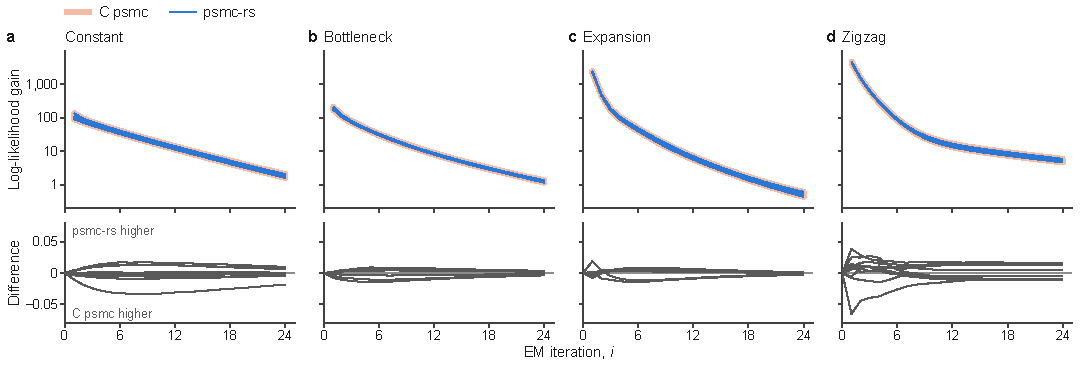
\includegraphics[width=183mm]{E1/figures/figS1_em_convergence.pdf}}
\caption{\textbf{C psmc and \psmcrs{} climb the same likelihood at every EM iteration (E1).} One column per simulated model, \EoneReps{} genomes each. Above: the log-likelihood gained in iteration~$i$, $\mathrm{LL}(i)-\mathrm{LL}(i-1)$, one line per genome and program (C psmc wide and pale underneath, \psmcrs{} thin and blue on top). All \EoneSoneGains{} gains were positive: the log-likelihood never decreased in either program, and in iteration~\EoneSoneLastIter{} it still rose by \EoneSoneGainLastMin{} to \EoneSoneGainLastMax{} units. Below: \psmcrs{}'s log-likelihood after iteration~$i$ minus C psmc's, one line per genome. From the same starting model ($i=0$) the two agreed within the rounding of the six decimals C psmc prints (at most \EoneSoneFirstAbsMax{}). After that they differed by at most \EoneSoneDiffMax{}; in each panel and iteration, the largest difference was at least \EoneSoneRatioMin{} times smaller than the smallest gain. After iteration~\EoneSoneLastIter{}, \psmcrs{}'s was the higher in \EoneSoneRsHigher{} of the \EoneGenomes{} genomes. Over all iterations, $\theta$ and $\rho$ of the two programs differed by at most a relative \EoneSoneThetaMax{} and \EoneSoneRhoMax{}. C psmc prints no log-likelihood after its last iteration, so the panels end at $i=\EoneSoneLastIter{}$.}
\label{fig:s1}
\end{figure}

\begin{table}[H]
\centering\small
\caption{\textbf{Accuracy of both programs, and their agreement, on simulated genomes (E1).} For each model, \EoneReps{} genomes of \EoneGenomeMb{}~Mb. Window: the informative window of the true model, 1\% to 99\% of its pairwise coalescence times. RMSE vs truth: each program's RMSE of $\log_{10}\Ne$ against the true history over the window (mean $\pm$ SD over the genomes). \psmcrs{} vs C psmc: $\Delta$, the RMSE of $\log_{10}\Ne$ between the two programs' fits, interval by interval over the window (median over the genomes), and the largest absolute difference $|d_k|$ in any interval of any genome (\suppmethods).}
\label{tab:s1}
\begin{tabular}{lrrrrrr}
\toprule
& \multicolumn{2}{c}{Window (years)} & \multicolumn{2}{c}{RMSE vs truth} & \multicolumn{2}{c}{psmc-rs vs C psmc} \\
\cmidrule(lr){2-3}\cmidrule(lr){4-5}\cmidrule(lr){6-7}
Model & from & to & C psmc & psmc-rs & $\Delta$ (median) & max $|d_k|$ \\
\midrule
Constant & 5,025 & 2,302,585 & 0.048 $\pm$ 0.023 & 0.048 $\pm$ 0.023 & \ensuremath{7.8\times10^{-6}} & \ensuremath{9.2\times10^{-5}} \\
Bottleneck & 10,050 & 1,322,585 & 0.291 $\pm$ 0.021 & 0.291 $\pm$ 0.021 & \ensuremath{3.9\times10^{-5}} & \ensuremath{6.6\times10^{-4}} \\
Expansion & 5,025 & 1,052,585 & 0.240 $\pm$ 0.043 & 0.240 $\pm$ 0.043 & \ensuremath{3.0\times10^{-5}} & \ensuremath{4.8\times10^{-4}} \\
Zigzag & 7,141 & 2,167,766 & 0.138 $\pm$ 0.013 & 0.138 $\pm$ 0.013 & \ensuremath{1.9\times10^{-5}} & \ensuremath{6.6\times10^{-5}} \\
\bottomrule
\end{tabular}

\end{table}

\begin{figure}[H]
\centering
\makebox[\linewidth][c]{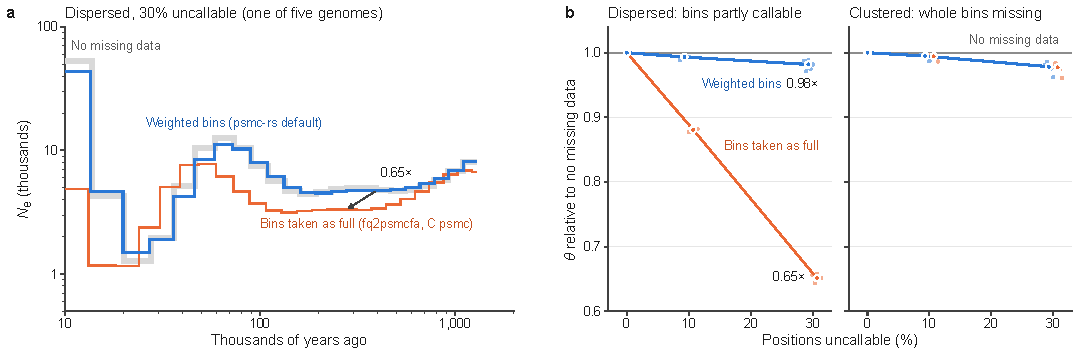
\includegraphics[width=183mm]{E4/figures/fig5_input_preparation.pdf}}
\caption{\textbf{Taking partly callable bins as full biases PSMC; weighting each bin by its callable bases removes most of the bias (E4).} We read \EfourRepsW{} simulated bottleneck genomes of \EfourGenomeMb{}~Mb without missing data, or from a VCF whose callable mask leaves 10\% or 30\% of positions uncallable in dispersed (mean run \EfourDispRunBp{}~bp) or clustered (mean run \EfourClusRunKb{}~kb) runs. Blue: \psmcrs{}'s default, each called bin weighted by its callable bases (\opt{--bin-callable auto}). Orange: C psmc's input, the bins \texttt{fq2psmcfa} makes from the consensus sequence, every called bin taken as full (fitted by \psmcrs{} with C psmc's model; Fig.~1). (a) One genome with the 30\% dispersed mask, the one whose weighted fit has the median RMSE against its fit without missing data, and that fit (wide grey), over the model's informative window; the arrow is the factor by which taking bins as full scales $\theta$, and with it every size and time. (b) $\theta$ relative to the fit of the same genome without missing data; large circles, medians, joined by lines and offset sideways so that both routes show where they agree (in the clustered facet the orange line, which would lie under the blue, is left out); small dots, replicates; numbers, the dispersed medians with 30\% missing. Dispersed runs leave many called bins with only part of their bases: about half (\EfourDispTenPartly{}) with 10\% missing and nearly all (\EfourDispThirtyPartly{}) with 30\%. Taken as full, they made $\theta$ \EfourDispTenFqTheta{} and \EfourDispThirtyFqTheta{} low, against \EfourDispTenAutoTheta{} and \EfourDispThirtyAutoTheta{} weighted. Clustered runs empty whole bins, which both models drop. Not drawn: multihetsep input, whose bins are taken as full, made $\theta$ \EfourDispThirtyMhsTheta{} low with 30\% dispersed and \EfourClusThirtyMhsTheta{} with 30\% clustered missing data; the VCF read without its mask, \EfourDispThirtyNomaskTheta{} and \EfourClusThirtyNomaskTheta{}. Simulations: $\mu=2.5\times10^{-8}$ per bp per generation, $g=25$ years.}
\label{fig:s2}
\end{figure}

\begin{figure}[H]
\centering
\makebox[\linewidth][c]{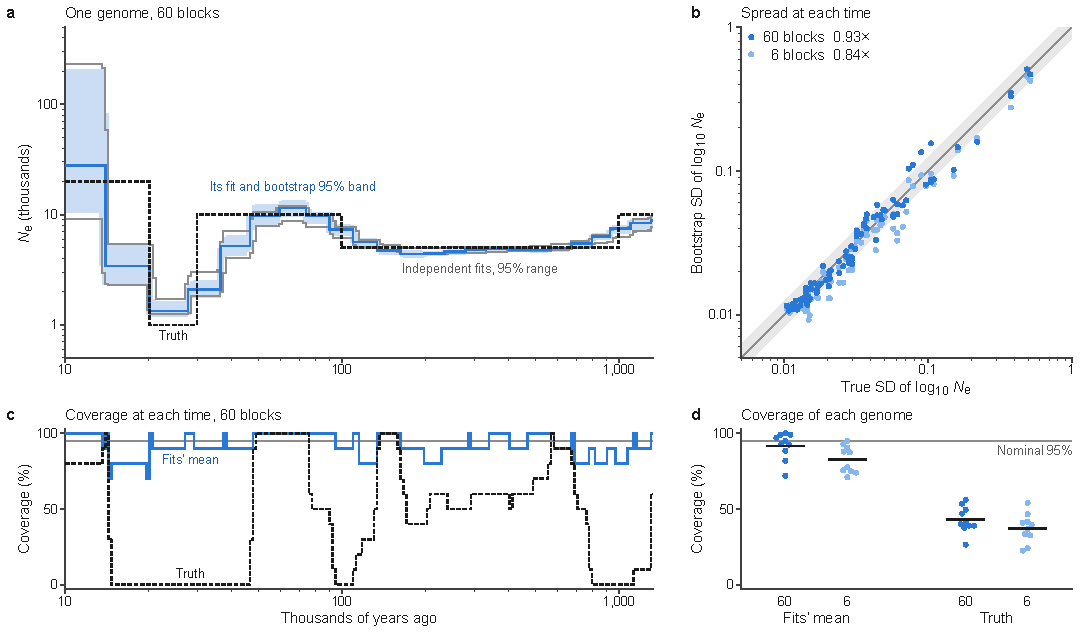
\includegraphics[width=183mm]{E5/figures/fig6_bootstrap_calibration.pdf}}
\caption{\textbf{The bootstrap measures the sampling variation of a PSMC fit, not PSMC's bias (E5).} The fits of \EfiveFits{} independent bottleneck genomes of \EfiveChroms{}$\times$50~Mb give the true sampling distribution of the estimate; \EfiveDatasets{} of them were bootstrapped (\EfiveReps{} replicates) in \EfiveFiveTrunks{} blocks of 5~Mb (blue) or \EfiveFiftyTrunks{} of 50~Mb (light blue); \EfiveFiveTrunks{} blocks is about what the default 50~Mb blocks give a 3~Gb genome. (a) One bootstrapped genome (\EfiveFiveTrunks{} blocks): its fit and bootstrap 95\% band, the truth (dashed) and, in grey, the 95\% range of the independent fits, over the model's informative window. (b) Bootstrap SD of $\log_{10}\Ne$ (median over the bootstrapped genomes) against the true SD, the SD over the independent fits, one dot per distinct pair of values over the window's times; grey line, identity; grey band, where a bootstrap SD equal to the true SD would fall, given the $\chi^2$ 95\% interval of an SD estimated from \EfiveFits{} fits; numbers, each block count's median ratio of the two SDs. (c) At each time, the share of the \EfiveDatasets{} bootstrapped genomes whose band (\EfiveFiveTrunks{} blocks) holds the fits' mean, their geometric mean (blue), or the truth (dashed). (d) The share of the window's times at which each genome's band holds the fits' mean or the truth; dots, genomes; bars, means. Grey lines in c and d, the nominal 95\%. The bands are nearly as wide as the fits' spread (bootstrap SD \EfiveFiveSd{} and \EfiveFiftySd{} times the true one, median over the window) but centred on a biased fit: PSMC smooths sudden changes in size, and the fits' median absolute bias, \EfiveBias{} in $\log_{10}\Ne$, was about twice their median SD, \EfiveSdTrue{}, so about as large as the half-width of a 95\% band. One demographic model was studied. Simulations: $\mu=2.5\times10^{-8}$ per bp per generation, $g=25$ years.}
\label{fig:s3}
\end{figure}
